Consider the scenario where one or more rogue agents (e.g., criminals) may be hiding in several isolated regions in a 2D workspace. To prevent them from potentially escaping from these regions to other nearby vulnerable regions, we may wish to set up line-of-sight sensors to detect if rogue agents attempt to escape. For the setup, a natural question one may ask is: what is the minimum number of line segments that are needed to form the desired barrier? The same setting finds many other practical applications, for example, for the identical setting, we may use the deployed sensors to track the movement of agents between different set of regions, e.g., understanding the flow of people between residential areas to commercial areas, which can benefit large-scale decision making, e.g., to help properly allocating resources for improving the city infrastructure. 
%
Alternatively, the computed line segments can serve as patrolling routes for autonomous agents (robots or humans) for actively monitoring intrusions, where the agents can always keep tracking events along the segments for which they are responsible.

%Barrier forming \cite{}, i.e. separating multiple sets of objects from each other,
%where each set may contain multiple scattered objects mix among other object sets, finds many real-world applications,
%e.g., erecting security fences around buildings,
%isolating different groups of agents (e.g., people, animals), 
%designing routes for patrolling robots to detect invaders, and so on. 
%multi-agent search for rouge agents, and so on. 
%These applications shares the common objective of better coverage or sensing of the environment with guards. 
%In reality, the types of barriers varies from barriers with range sensibility like lidar, visibility-based barriers like cameras or guards, to physical straight line fences or walls.
%
Motivated by the above stated scenarios and inspired by earlier research in robotics on barrier forming \cite{kloder2007barrier,kloder2008partial}, i.e., erecting barriers for separating regions of interest, in this paper, we examine the variation of finding the minimum number of straight line segments for isolating multiple sets of points of polygons in a two-dimensional workspace. Fig~\ref{fig:ex}[left] illustrates an instance where three colored polygonal sets are to be separated from each other and the grey polygons are obstacles. Fig~\ref{fig:ex}[right] shows a possible solution which is fairly non-trivial 
to obtain. 
%
%The problem finds applications in many practical scenarios where geometric separation is needed, for example, the deployment of a minimum set of  line-of-sight security beams to guard critical areas from intrusions. 
%dividing different rooms in a floor or buildings from each other to prevent the %spread of virus or contagious diseases,
%designing the surveillance routes for guards that walk on a straight route,
%building fences for regions among different security level that are not allowed 
%to have connections, and so on. 

\begin{figure}[t]
    \centering
    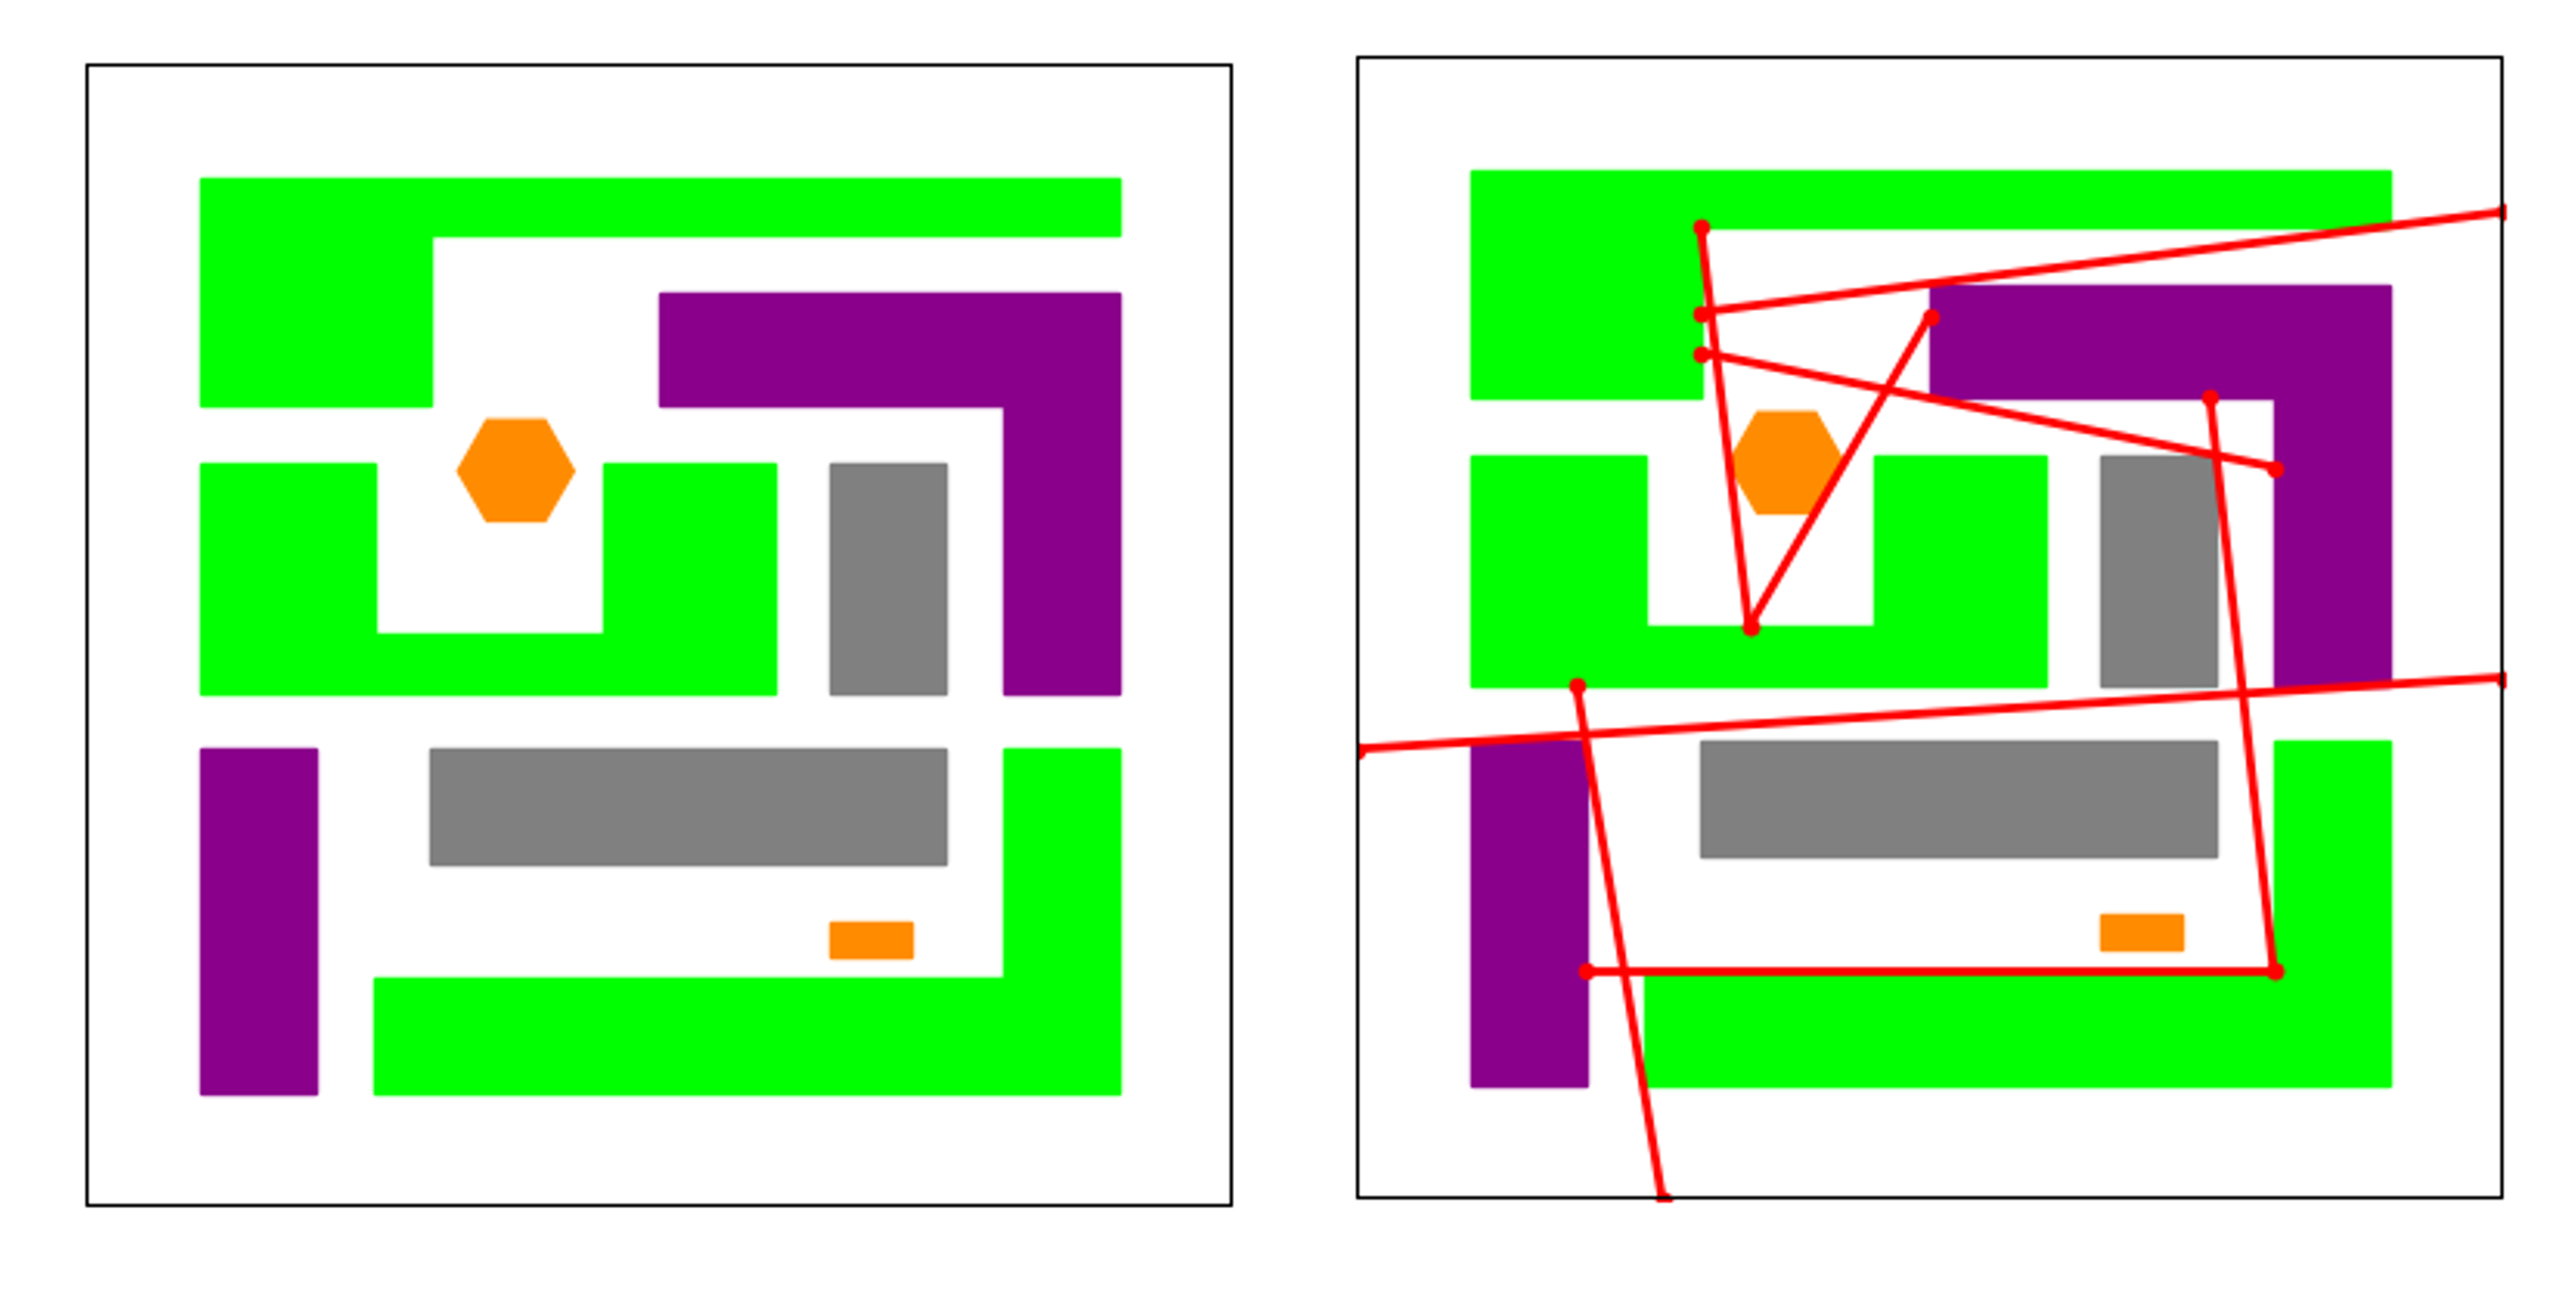
\includegraphics[width=\columnwidth]{chapters/bc/fig/intro_pic.png}
    \caption{Example of barrier forming for separating three sets of complex polygonal shapes. Different colors represent different sets with the grey ones representing obstacles. The red line segments are the barriers computed by our algorithm.}
    \label{fig:ex}
    \vspace{-0.2in}
\end{figure}
As a summary of this work and its contributions, we study three settings in using line segments to separate sets of disjoint geometric shapes in a 2D workspace: (1) separating point sets, (2) separating point sets among polygonal obstacles, and (3) separating polygonal sets among polygonal obstacles. 
%
Whereas all three settings are NP-hard to optimally solve, we derive an effective method for computing optimal solutions for the first two settings, capable of handling tens of objects (points and/or polygons) partitioned into multiple sets. 
%
The  method first systematically computes candidate barrier set containing a minimum separating barrier, and then builds a novel integer programming model for finding the minimum barrier. 
%
Following a similar approach, we also develop a method that computes solutions for the third setting that is proven to be at least $2$-optimal. 
%
We provide theoretical analysis that shed some light on why the setting involving polygonal sets is more difficult to solve.
%
Extensive simulation study corroborates the effectiveness of our algorithms. 

%Our contribution to barrier forming is, in summary, formulating the problem of minimizing
%the line segment barriers used with respect to different kinds of object sets (point object and polygonal object). 
%For barrier forming among sets of point objects, we provide effective integer programming based method to obtain the optimal solution.
%For the general polygonal objects, our method can provide a guaranteed 2-OPT solution.
%We also perform evaluations on four different settings to show
%the effectiveness of the proposed method.


\noindent\textbf{Related Work}.
Our investigation of barrier forming has its origins from several research areas.
In the study of pursuit evasion or more generally differential games \cite{ho1965differential,isaacs1999differential,hajek2008pursuit,tovar2009sensor,simov2000pursuit,guibas1997visibility,kameda2006online,kirousis1986searching, wen2018localization, sachs2004visibility,lau2005optimal, yu2011shadow, olsen2022robust}, 
% flash light searcher, 1-2 inf searcher
such scenarios often happen where several agents are tasked to search an environment for hidden rogue agents or to protect critical regions from outsider invaders, which amount to creating and maintaining static or dynamic barriers of some form.  
%
Among the approaches taken in finding solutions for these problems, some resort to discretize the environment into graph representations and conduct search over them \cite{kirousis1986searching, sachs2004visibility}, while others adopt probabilistic reasoning \cite{lau2005optimal, yu2011shadow}. 
%
In particular, Tovar et al. \cite{tovar2009sensor} studied a problem that examines how to untangle sensor beam crossings to reason about the state of a robot, and use the insight to build algorithms for driving a robot to a desired state. In a sense, their study can be viewed as studying a problem that is a dual of the problem that we study here. 

%\textcolor{red}{JJ's edit location}

Barrier forming problems can also be seen as a type of sensor coverage problem. 
%
A series of study of perimeter defense/guarding problems aim at covering the boundaries of some regions to protect them from the outside \cite{shishika2020cooperative, macharet2020adaptive, FenHanGaoYuRSS19, FenYuRSS20}, which share similar motivations. 
The barrier forming problem has more flexible solutions by not fixing the specific boundaries to secure for the critical regions,
which can be more general and closer to reality.
In \cite{kloder2007barrier}, the authors solved the barrier coverage problem optimally under non-trivial environment to minimize the total length of the barriers between two groups of polygonal objects. 
To tackle the proposed problem, a novel and efficient network-flow based method is applied. 
In \cite{abrahamsen2020geometric}, the work is extended to multiple groups of objects.
The following work \cite{kloder2008thesis} includes a similar problem formation to the problem studied in this paper, where the objective is minimizing the number of fixed-length line segments used. 
%
However, that proposed method in \cite{kloder2008thesis} uses Tarski sentence \cite{tarski1949decision} which, to our knowledge, does not have very effective method.


This work is closely related to several problems in computational geometry, especially point set shattering which seeks a complete separation among a single set of points \cite{freimer1991complexity, har2020separating}. 
Bichromatic point sets or polyherdral separation problem uses wedges, axis-aligned lines, chords, parallel lines, or circles to separate two sets of points or polyhedra \cite{devillers2001separating,armaselu2017geometric,boissonnat2001circular, demaine2005separating}. 
Work on these problems often put on specific constraints such as working with convex objects or simple polygons without holes, adopting non-crossing or parallel lines as the separator, and so on. 

\noindent \textbf{Paper Structure}.
The rest of the paper starts with formulating the barrier formation problem and introducing the three variants studied in Section~\ref{sec:preliminary}. 
Then, we describe the structure analysis of the problem in Section~\ref{sec:structure}, which will base the algorithm
proposed in Section~\ref{sec:algorithm}. Lastly, in Section~\ref{sec:evaluation} we evaluate the algorithm on four different scenarios. %\r{associate each with a specific section.}

%  methods take
% The problem of constructing a set of barriers appears in various robotics applications 


% Barrier forming is studied in various domains.
% In the pursuit evasion game, barriers were constructed to perform 
% area scan, moving target persuasion \cite{yu2011shadow, tovar2009sensor} etc.
% In computational geometry,
% barrier forming has relevance to several problem: 
% Regarding separating polygons, 
% the study of barrier coverage problem introduces a network flow-based algorithm 
% for computing the minimum total distance separation for two sets of polygons 
% with the existence of obstacles\cite{kloder2007barrier, kloder2008thesis}.
% In \cite{kloder2008thesis}, the author explored barrier forming with minimum number of 
% fixed-length line segments, while it is still important to find high performance
% solution for such problem.